\documentclass[12pt]{article}

% Misc. packages
\usepackage{fancyvrb}
\usepackage{url}
\usepackage{hyperref}
\usepackage{authblk}
\usepackage{geometry}
\usepackage{enumerate}

% Math & Symbol packages
\usepackage{mathtools,bm}
\usepackage{amsmath,amsfonts,amssymb}   %% AMS mathematics macros
\usepackage{amsmath}
\usepackage{amssymb}

% Graphics & Float packages
\usepackage{float}
\usepackage{graphicx}
%\usepackage{subfigure}
\usepackage{tikz}
\usepackage{pgfplots}
\pgfplotsset{compat=newest}

% Tikz and pgfplots libraries
\usetikzlibrary{patterns, arrows.meta, calc}
\usepgfplotslibrary{fillbetween}

% Colors
\usepackage{xcolor}
\definecolor{lightblue}{rgb}{0.0,0.5,0.8}
\definecolor{HMSRed}{HTML}{C5112E}  % [197, 17, 46]
\definecolor{MGHBlue}{HTML}{008BB0} % [0, 139, 176]
\definecolor{MGHGrey}{HTML}{626365} % [98, 99, 101]

% Annotation commands
\newcommand{\todo}[1]{{\color{lightblue}\par {[{\bf TO DO: } {\em #1}} ] \\    }}
\newcommand{\addref}[1]{{\color{red}{\bf [REF #1]}}}
\newcommand{\MPKcomment}[1]{{\color{magenta}\par {[{\bf MPK: } { #1}} ] \\    }}
\newcommand{\DCcomment}[1]{{\color{magenta}\par {[{\bf DC: } { #1}} ] \\    }}
\newcommand{\KvAcomment}[1]{{\color{magenta}\par {[{\bf KvA: } { #1}} ] \\    }}

% Document formatting
\linespread{1.4}
\geometry{
a4paper,
total={174mm,257mm},
left=20mm,
top=20mm,
}
\renewcommand{\floatpagefraction}{.8}
\renewcommand\Affilfont{\fontsize{9}{10.8}\itshape}

%~~~~~~~~~~~~~~~~~~~~~~~~~~~~~~~~~~~~~~~~~~~~~~~~~~~~~~~~~~~~~~~~~~~~~~~~~~~~~~~~~~~~~~~~~~~~~~~~~%
\title{Solving the dynamic fluence map sequencing problem using piecewise linear leaf position and dose rate functions}
%\title{Dynamic leaf sequencing via trajectory representations of leaf trajectories and dose rate}

\author{Matthew Kelly, Koos van Amerongen, David Craft}
\affil[]{Department of Radiation Oncology, Massachusetts General Hospital, Harvard Medical School}
%% \date{February 13, 2016}  % Comment to use today's date

\begin{document}

\maketitle
\thispagestyle{empty}

\begin{abstract}
  Within the setting of intensity modulated radiation therapy (IMRT) and the fully continuous version of IMRT called
  volumetric modulated radiation therapy (VMAT), we consider the problem of matching a given fluence map $f$ as well as possible in
  limited time $T$ by the use of a multi-leaf collimator (MLC).
  We use linear splines for leaf position and the dose rate as functions of time.
  The optimization computes the dose rate and leaf trajectories that best produce
  the target fluence map.
  Computing the dose rate and leaf trajectories is a non-convex optimization problem
  with many local minima.
  In our optimization we use a smooth model of how the leaves block the fluence radiation,
  which helps speed computation and avoid local minima.
  We solve the optimization in two parts:
  an outer optimization loop that optimizes the dose rate pattern over time, and 
  an inner optimization loop that--given a fixed dose rate pattern--optimizes the leaf trajectories.
\end{abstract}

\section{Introduction}
The dynamic delivery of a given fluence map by a multi-leaf collimator (MLC) remains a difficult, largely unsolved problem.
The sliding-window leaf-sweep algorithm (SWLS) \cite{leafsweep}, 
    in which the MLC leaves cross the treatment field in a unidirectional fashion, 
    achieves perfect fluence map replication if sufficient time is available \cite{Stein94}.
However, the SWLS algorithm is not in general efficient with respect to the required delivery time.
Time is an important aspect of VMAT and IMRT treatment plans, for several reasons:
\begin{enumerate}[i)]
  \item The effect of patient movement on delivery inaccuracy increases in the time the patient is exposed to radiation.
  \item Shorter treatments allow the treatment facility to help more patients on a given set of radiation therapy machines, 
        which is particularly relevant to third-world countries as these machines are expensive.
  \item In general, there is a trade-off between dose quality and delivery time, and given how widespread the use of radiation therapy is in treating cancer, it makes sense to put in effort to assure that we are on the Pareto optimal frontier regarding these two objectives.
  
\end{enumerate}
Several studies have investigated the trade-off between treatment time and plan quality \cite{tradeoffSalari,tradeoffMCO,tradeoffCraft}.
\cite{balvertcraft} were the first to include treatment time in the leaf sequencing step of the treatment plan optimization challenge.
They construct the trade-off curve between delivery time and fluence map matching accuracy by optimizing leaf trajectories and dose rate patterns for a sequence of delivery times.
% for several leaf trajectories independently
For a given fluence map and fixed delivery time, the challenge of optimizing the leaf trajectories and dose rate versus time so that the given fluence map is matched as accurately as possible, subject to machine restrictions, presents a large scale nonconvex optimization problem.
The nonconvexity of the fluence map matching problem leads to a large number of local minima.
For a thorough introduction to the complexities of dynamic fluence map delivery (which generally arises in the context of dynamic IMRT and VMAT),
 see \cite{balvertcraft} and \cite{unkvmatreview}.

\section{Model}
We assume we start with a fluence map $m$
that has been optimized, along with additional fluence maps located around the patient, to collectively yield a dose distribution optimized for the particular patient's geometry (location of tumor and all nearby organs) and dose prescription. We do not model this aspect of the problem and simply assume that the optimal fluence maps are given. The algorithms set forth in this paper determine how to construct the given fluence map by moving the leaves of the MLC across the field (back and forth if necessary; unidirectionality is not imposed, and in fact it is known that enforcing unidirectionality can be suboptimal, see the Appendix of \cite{balvertcraft}) while varying the dose rate.

We assume the fluence map $m$ is given as a matrix where the rows correspond to the individual left and right leaf pairs, and the columns are the discretely optimized fluence bixels across the field, which can be as finely discretized as one wishes, but typical length scales are on the order of 0.5 cm for the row height of the MLC leaves, with the same value used for the across the row discretization. 

Let $x^i_L(t)$ and $x^i_R(t)$ denote the leaf position of the $i$th left and right leaves respectively, at time $t$.
Our framework puts the dose rate optimization in an outer loop. For a given dose rate over time profile, the leaf rows can be optimized independently (neglecting the small coupling terms created by the tongue-and-groove mechanism on the real machine, see \cite{unkvmatreview}), so for the remainder of the algorithm development, we consider only a single leaf row.

Let the fluence row that we are considering from the $m$ matrix be given as a continuous function $f(x)$, where $x$ is the location across the fluence row. Note that $f(x)$, if it derives directly from a row $i$ of the matrix $m$, will be a piecewise constant function, but in general $f(x)$ could also be a smooth function of $x$. We typically think of a smooth function $f(x)$ since the piecewise constant version is simply an artifact of the fact that the dose optimization is done discretized.

We assume the total allowed treatment delivery time $T$ is given. Our goal is then to compute leaf trajectories $x_L(t)$ and $x_R(t)$ as well as a dose rate $d(t)$ to recreate the fluence map row $f(x)$ as best as possible.

The fluence achieved at each position $x$, $g(x)$, is the time-integral of the dose rate for the times that position is exposed.
This time domain $\mathcal{T}(x)$ is the set of times when the position $x$ is not blocked by either of the leaves, i.e.,
$\mathcal{T}(x)$ is the set of all times $t$ such that $x_L(t) \le x \leq x_R(t)$,
as illustrated by Figure \ref{fig:administeredDose} .

\begin{equation}
g(x) = \int_{\mathcal{T}(x)} d(t) dt
\label{eqn:deliveredFluenceDose}
\end{equation}

Our goal is to find the leaf trajectories $x_L(t)$ and $x_R(t)$ and dose rate pattern $d(t)$
that minimize the squared integral error between the target fluence $f(x)$ and the delivered fluence $g(x)$:

\begin{equation}
\underset{d(t), \, x_L(t), \, x_R(t)}{\operatorname{argmin}}
\int_X \bigg(f(x)) - g(x)\bigg)^2 dx .
\label{eqn:fluenceMapOptimization}
\end{equation}

% KvA: Example Figure, didn't care too much about efficiency
\begin{figure}[htp]
\centering
    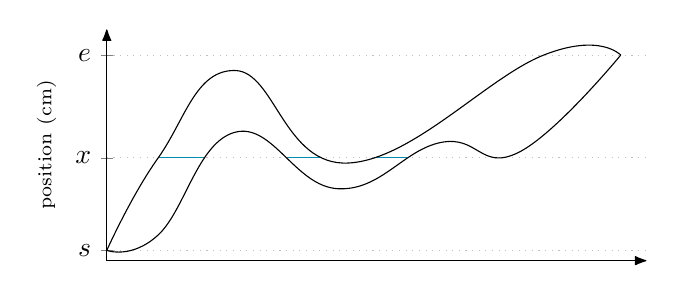
\begin{tikzpicture}[remember picture]
        \pgfplotsset{holdot/.style={color=black,only marks,mark=*,mark size=1.5pt}}
        \pgfplotsset{soldot/.style={color=white,only marks,mark=*,mark size=1.5pt}}
        \begin{axis}[
            xmin=0, xmax=10.50,
            ymin=0, ymax=4.5,
            grid = both,
            grid style = dotted,
            axis x line = bottom,
            axis y line = left,
            enlargelimits = {abs=0.0},
            axis line style = {-Latex[round]},
            yticklabels = {$s$,$x$,$e$},
            ytick = {0.2,2,4},
            xtick = \empty,
            ylabel = {\scriptsize{position (cm)}},
            axis equal image
        ]

            % Vertical lines (top)
            \node[] (traj-1) at (axis cs:1,4.2) {};
            \node[] (traj-2) at (axis cs:1.88,4.2) {};
            \node[] (traj-3) at (axis cs:3.5,4.2) {};
            \node[] (traj-4) at (axis cs:4.17,4.2) {};
            \node[] (traj-5) at (axis cs:5.2,4.2) {};
            \node[] (traj-6) at (axis cs:5.85,4.2) {};
            \node[] (traj-10) at (axis cs:10,4.2) {};

            % Exposure times
            \draw[MGHBlue] (1,2) -- (1.89,2);
            \draw[MGHBlue] (3.5,2) -- (4.17,2.0);
            \draw[MGHBlue] (5.2,2) -- (5.85,2);

            % Leaf trajectories
            \addplot[name path global = leafl, black, smooth, tension=0.75] coordinates{(0,0.2)(1,2)(2.5,3.7)(4.7,1.9)(8.5,4)(10,4)};
            \addplot[name path global = leafr, black, smooth, tension=0.75] coordinates{(0,0.2)(1,0.5)(2.5,2.5)(4.5,1.4)(6.5,2.3)(8,2.1)(10,4)};

        \end{axis}
    \end{tikzpicture}

    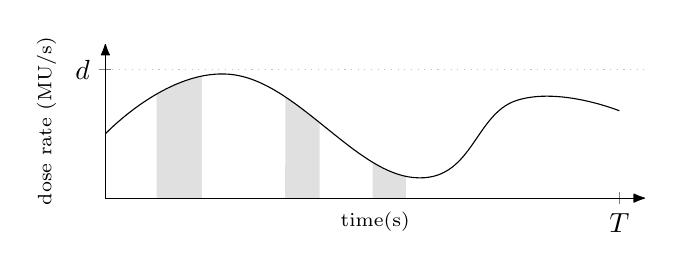
\begin{tikzpicture}[remember picture]
        \pgfplotsset{holdot/.style={color=black,only marks,mark=*,mark size=1.5pt}}
        \pgfplotsset{soldot/.style={color=white,only marks,mark=*,mark size=1.5pt}}
        \begin{axis}[
            xmin=0, xmax=10.50,
            ymin=0, ymax=3.0,
            ymajorgrids = true,
            grid style = dotted,
            axis x line = bottom,
            axis y line = left,
            enlargelimits = {abs=0.0},
            axis line style = {-Latex[round]},
            xticklabels = {$T$},
            xtick = {10},
            yticklabels = {$d$},
            ytick = {2.5},
            xlabel style = {at={(ticklabel* cs:0.5,1.5)},anchor=north},
            xlabel = {\scriptsize{time(s)}},
            ylabel = {\scriptsize{dose rate (MU/s)}},
            axis equal image
        ]

            % Vertical lines (bottom)
            \node[] (dose-1) at (axis cs:1,-0.2) {};
            \node[] (dose-2) at (axis cs:1.88,-0.2) {};
            \node[] (dose-3) at (axis cs:3.5,-0.2) {};
            \node[] (dose-4) at (axis cs:4.17,-0.2) {};
            \node[] (dose-5) at (axis cs:5.2,-0.2) {};
            \node[] (dose-6) at (axis cs:5.85,-0.2) {};
            \node[] (dose-10) at (axis cs:10,-0.2) {};

            % Dose rate pattern
            \addplot[name path global = dose, black, smooth, tension=0.75] coordinates{(0,1.25)(2.5,2.4)(6,0.4)(8,1.9)(10,1.7)};\
            \addplot[name path global = xaxis, draw=none, domain=0:11] {0};

            % Integrals
            \addplot [thick, color=blue, fill=MGHGrey, fill opacity=0.2]
                fill between[of=xaxis and dose, soft clip={domain=1:1.88}];
            \addplot [thick, color=blue, fill=MGHGrey, fill opacity=0.2]
                fill between[of=xaxis and dose, soft clip={domain=3.5:4.17}];
            \addplot [thick, color=blue, fill=MGHGrey, fill opacity=0.2]
                fill between[of=dose and xaxis, soft clip={domain=5.2:5.85}];

            % Correction
            \addplot[fill = white]
                fill between[of=xaxis and dose, soft clip={domain=1.88:2}]; % filling
            \addplot[fill = white]
                fill between[of=xaxis and dose, soft clip={domain=4.17:4.5}]; % filling
            \addplot[fill = white]
                fill between[of=xaxis and dose, soft clip={domain=5.85:6}]; % filling
             \draw[black] (0,0) -- (10,0);

        \end{axis}
    \end{tikzpicture}

    \begin{tikzpicture}[remember picture,overlay]
        \draw[dashed,MGHGrey!60] (traj-1) -- (dose-1);
        \draw[dashed,MGHGrey!60] (traj-2) -- (dose-2);
        \draw[dashed,MGHGrey!60] (traj-3) -- (dose-3);
        \draw[dashed,MGHGrey!60] (traj-4) -- (dose-4);
        \draw[dashed,MGHGrey!60] (traj-5) -- (dose-5);
        \draw[dashed,MGHGrey!60] (traj-6) -- (dose-6);
        \draw[dashed,MGHGrey!60] (traj-10) -- (dose-10);
    \end{tikzpicture}

\vspace{-0.7cm}
\caption[Illustration of administered dose]{
    Illustration of administered dose: the dose administered to a position $x$ equals the integral (shaded area) of the dose rate (lower panel) over the moments in time (blue lines) that position is exposed by the leaves (upper panel).
    }
\label{fig:administeredDose}
\end{figure}



\section{Solution approach}

With the problem we are trying to solve now formally stated as an optimization problem, we turn
to the solution approach. The first step in this is to turn the integral problem statement into
a format suitable for solution by a continuous optimization solver such as 
FMINCON \cite{MatlabOptimizationToolbox2014}, SNOPT \cite{Snopt7}, or IPOPT \cite{Wachter2006}.
This requires two main steps: determining a suitable numerical representation of the control variables, the leaf positions and doe rate as a function of time, and then using this representation
to form a well-defined optimization problem (which in this case amounts to solving the intergral
in Equation \ref{eqn:deliveredFluenceDose}.

\subsection{Spline representation}

We represent each of the three time functions we are optimizing for
by piecewise linear splines. Each of the three trajectories shares the same set of knot times $t_k \in \{t_0, t_1, \dots, t_N\}$, where $N$ is the number of knot points. We denote the value of the leaf positions and dose rate at knot time $t_k$ by $x_{L,k}$, $x_{R,k}$, and $d_k$. 

\begin{figure}
  \centering
  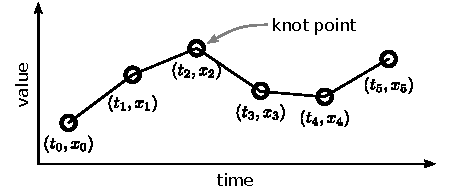
\includegraphics{fig/linearSpline.pdf}
  \caption{Linear Spline. We represent the dose rate and leaf position trajectories as linear splines. A linear spline is fully defined by its values at the knot points. }
  \label{fig:linearSpline}
\end{figure}

\subsection{Integral computation with blocking function $k$}

We now need to evaluate the integral $g(x)$, Equation \ref{eqn:deliveredFluenceDose} from the spline representation.
There are two issues with computing this integral directory.
The first is that it requires either computing the inverse of the leaf trajectories (in order to figure out the times that the leaves pass each position of interest), which
ultimately reduces to a non-linear root finding sub-problem. When placed inside of an optimization, this will dramatically slow convergence.
The second issue is that the set $\mathcal{T}(x)$ does not smoothly vary with respect to the leaf trajectories.
%It is possible to construct a set of leaf trajectories for which a small change in leaf position
%switches $\mathcal{T}(x)$ from one to two simply connected sets.
Inside of an optimization, this would cause a change in the sparsity pattern of the gradient
(\textit{e.g.} $\tfrac{\partial g}{\partial x_L})$)
between successive iterations,
which leads to poor convergence and possibly numerical instability.

Our solution is to rewrite the integral using a blocking function $k(t,x)$, which has a value of one when the leaves at time $t$ are passing radiation at location $x$ and zero when the leaves are blocking radiation. This allows us to rewrite the integral using the constant bounds $[0, T]$:

\begin{equation}
  g(x) = \int_0^T \! k(t, x) \cdot d(t) \, dt
  \label{eqn:fluenceDoseSimpleBounds}
\end{equation}

Now we have a standard scalar integral and we can use any quadrature method to evaluate (\ref{eqn:fluenceDoseSimpleBounds}).
In our case we use the midpoint (rectangle) quadrature rule. 

As just defined, our fluence blocking function $k(t,x)$
would also have a discontinuous gradient, which would cause problems in the optimization.
Therefore, we use the exponential sigmoid functions to approximate the step function
$s(x, \alpha) = \frac{1}{1 + e^{-x \alpha}}$, where $\alpha$ is the smoothing parameter. A smaller smoothing parameter will provide a more accurate model, while a larger smoothing parameter will lead to faster optimization. With this approximation to the step function in hand, we have that

\begin{equation}
  k(t, x) \approx \sqrt{s\big(x_L(t) -x, \, \alpha\big) \; \cdot \; s\big(x -x_R(t), \, \alpha\big)}
\end{equation}
since for a position $x$ to be exposed, it needs to be exposed by {\em both} left and right leaves.

In practice it is useful to define the $\alpha$ in terms of a smoothing distance $\Delta x$ and the
value $\gamma$ of the smoothing function at a distance $\Delta x$ from the boundary. For example, $\Delta x = 0.05$ cm and $\gamma = 0.98$ means that at a distance of 0.05 cm from the edge of the leaf, it is blocking 98\% of the radiation, and at a distance of -0.05 cm it is blocking 2\% of the radiation.

\begin{equation}
  \alpha = \frac{-\ln(1-\gamma)}{\Delta x}
  \label{eqn:SmoothingDistanceParameter}
\end{equation}

\subsection{Objective Function}

The objective function for the inner optimization (computing leaf trajectories)
is the integral of the error-squared between the desired fluence $f(x)$ and the fluence that
is delivered by the current set of trajectories, $g(x)$.
\begin{equation}
  J = \int_{x_\text{min}}^{x_\text{max}} \! \bigg( f(x) - g(x) \bigg)^2 \,dx
  \label{eqn:continuousFittingObjective}
\end{equation}

In practice we can only compute the fluence profile at a finite number of points. We will break the domain $[x_\text{min}, x_\text{max}]$ into $N_\text{fit}$ equal-width segments,
and evaluate the fluence target and delivered fluence at the midpoint $x_k$ of each segment.

\begin{equation}
  J \approx \frac{x_\text{max} - x_\text{min}}{N_\text{fit}}
  \sum_{k = 1}^{N_\text{fit}} \! \bigg( f(x_k) - g(x_k) \bigg)^2
  \label{eqn:discreteFittingObjective}
\end{equation}

\subsection{Computing Leaf Trajectories as a Non-linear Program}
\label{sec:LeafTrajectoryAsNLP}

The inner optimization loop computes the leaf trajectories $x_L(t)$ and $x_R(t)$
that minimize the objective function (\ref{eqn:continuousFittingObjective})
and satisfy the position and velocity constraints given below.

The limits on leaf position can be implemented as a combination of
constant bounds and linear inequality constraints:

\begin{equation}
  x_\text{min} \leq x_{L, k}
  \quad \quad
  x_{R, k} \leq x_\text{max}
  \quad \quad
  x_{L, k} \leq x_{R, k}
  \quad \quad
  \forall k
  \label{eqn:PositionLimits}
\end{equation}

The trajectories as piecewise linear splines, represented here by their values at the knot points $t_k$.
The velocity trajectory can easily be computed by taking the derivative of the spline:.

\begin{equation}
  \dot{x}_{L, k} = \frac{x_{L, k+1} - x_{L, k}}{h_k}
  \quad \quad
  \dot{x}_{R, k} = \frac{x_{R, k+1} - x_{R, k}}{h_k}
\end{equation}
\noindent where $h_k$ is the distance between knot point $k$ and $k+1$ (we use equal spacing for all knot points).

The limits on velocity can thus be written as linear inequality constraints:

\begin{equation}
  -v_\text{max} \leq \dot{x}_{L, k} \leq v_\text{max}
  \quad \quad
  -v_\text{max} \leq \dot{x}_{R, k} \leq v_\text{max}
  \quad \quad \forall k
  \label{eqn:VelocityLimits}
\end{equation}

\DCcomment{MATT I'm wondering if we need one more word here that describes going from
the knot points to the smoothed k function to the g integral (any details that are of interest/might
not be entirely obvious?).} 

\subsection{Iterative refinement of smoothing parameter}

In practice, the leaf trajectory optimization runs well (\S\ref{sec:LeafTrajectoryAsNLP})
when the smoothing distance $\gamma$ (\ref{eqn:SmoothingDistanceParameter}) is large.
As the smoothing becomes smaller, the optimization becomes more difficult to solve,
but the model is more accurate.

We can use these properties to our advantage by iteratively solving the optimization problem.
On the first iteration we use a large value for the smoothing parameter,
which will quickly find a good approximation of the solution.
On subsequent iterations we use the solution from the previous optimization as the initial guess,
and then reduce the smoothing parameter until we achieve the desired model accuracy.

This process is reasonably effective at avoiding local minima:
the optimization with heavy smoothing has few issues with local minima, finding a good global solution.
Subsequent optimizations are similar, so the previous solution is an excellent guess,
and the optimization is able to simply refine that solution for the more accurate model.

%~~~~~~~~~~~~~~~~~~~~~~~~~~~~~~~~~~~~~~~~~~~~~~~~~~~~~~~~~~~~~~~~~~~~~~~~~~~~~~~~~~~~~~~~~~~~~~~~~%

\subsection{The outer loop: computing the dose rate trajectory}
We handle the outer loop master problem, which optimizes the dose rate over time, by a
global optimization procedure since starting from any fixed dose rate pattern and optimizing with
a smooth gradient-based solver, as is done for the leaf trajectories, yileds with near certainty
a local minima that is far from optimal.

We use the CMAES algorithm \cite{Hansen2001}, which
works by widely sampling the objective function (dose rate trajectory knot points in our case) and then fitting a multi-variate Gaussian to the value of the objective at those points.
Then it samples new points from that Gaussian and updates the model.
Since CMAES does not require explicit gradient calculations, it tends to be more robust to problems
with many local minima and complex objective functions.


\section{Results}

In this section we present a collection of simple experiments to demonstrate various features of the
proposed algorithm.

\todo{Recompute the plots in this section to be consistent with new definition of the smoothing
      parameter.}

\subsection{Smoothing Comparison}
\label{sec:LeafSmoothingComparison}

In Section \S\ref{sec:modelingFluenceBlocking} we describe a smooth model of how the leaves block radiation.
Here we describe do a simple experiment to look at how adjusting that smoothing parameter affects the optimization.

We uses a single target fluence profile, as shown in Figure \ref{fig:fluenceMapSmoothingExample},
and assumes that the dose rate is a constant function of time.
We performed a simple grid search, computing the optimal leaf trajectories for each dose rate value.
We then ran this grid-search twice, once with heavy smoothing and once with light smoothing.

The smoothing parameter can be expressed in terms of a characteristic blurring width.
Here we used a width of 0.5 cm for the heavy smoothing and 0.05 cm for the light smoothing.
The characteristic width was computed such that the smoothing function achieved 95\% of its
change in value over the smoothing window.

We also used seven of leaf trajectory segments, although similar results are obtained for trajectories with more segments.
\todo{add a figure for that? Or maybe another sub-section?}
This number was computed with a pilot study.
Fewer trajectory segments lead to faster solve times, but the fitting error increases significantly.
Using more trajectory segments takes longer, but at a trivial reduction in fitting error.

Figure \ref{fig:smoothVsStiffOptimization} shows the two sequences of optimizations, one for the
heavy smoothing of 0.5 cm and the other for the light smoothing of 0.05 cm.
The objective function is normalized by the fitting error associated with a solution where the
leaves completely block the radiation.
Although both optimizations are able to find reasonable solutions, there are a few salient differences.
The optimization with light smoothing takes about four times longer to run when
compared to the optimization with heavy smoothing.
The optimization with light smoothing also tends to get stuck in local minima, as shown by the
objective function jumping around with small changes in the constant dose rate.
The optimization with heavy smoothing eventually converges to trajectories that rely on the
smoothing behavior to achieve the desired fluence profile. This is clear from the discrepancy
between the smooth and exact model for dose rates above 4 MU.
That being said, this discrepancy between the models is small and the overall shape of the delivered
fluence map is generally correct, as shown in Figure \ref{fig:smoothVsStiffOptimization}.

\begin{figure}
  \centering
  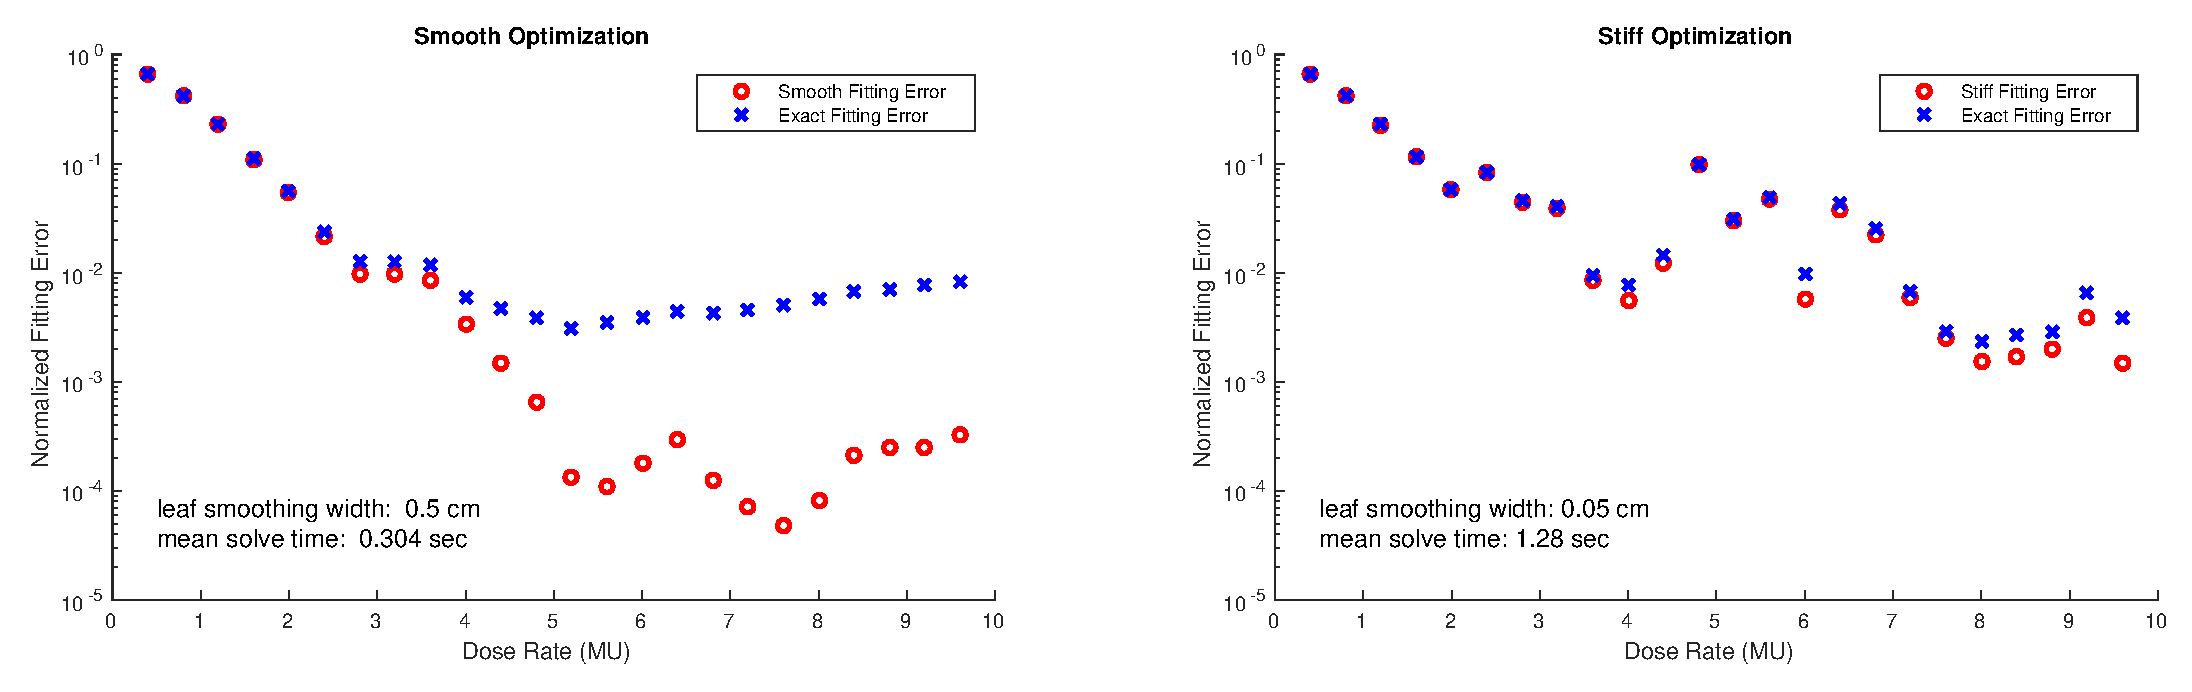
\includegraphics[width=\textwidth]{fig/smoothVsStiffOptimization.pdf}
  \caption{Comparison of heavy and light smoothing in leaf-blocking model.
           In each plot we ran 24 leaf optimizations, sweeping through a range of constant dose rate trajectories.
           The optimizations in the left plot used a leaf smoothing distance of 0.5 cm, while the
           right plot used 0.05 cm.
           Notice that the left set of optimization does a better job of avoiding local minima,
           but that there is a disparity between the fluence profile produced by the smooth model
           and the exact (no smoothing) model.
           The right plot does better job of matching the exact model, but it tends to get stuck in local minima
           and takes significantly (4x) longer to run.
           The solution for a dose rate of 5.2 MU on the left plot is
           shown in detail in Figure \ref{fig:fluenceMapSmoothingExample}.
          }
  \label{fig:smoothVsStiffOptimization}
\end{figure}

\begin{figure}
  \centering
  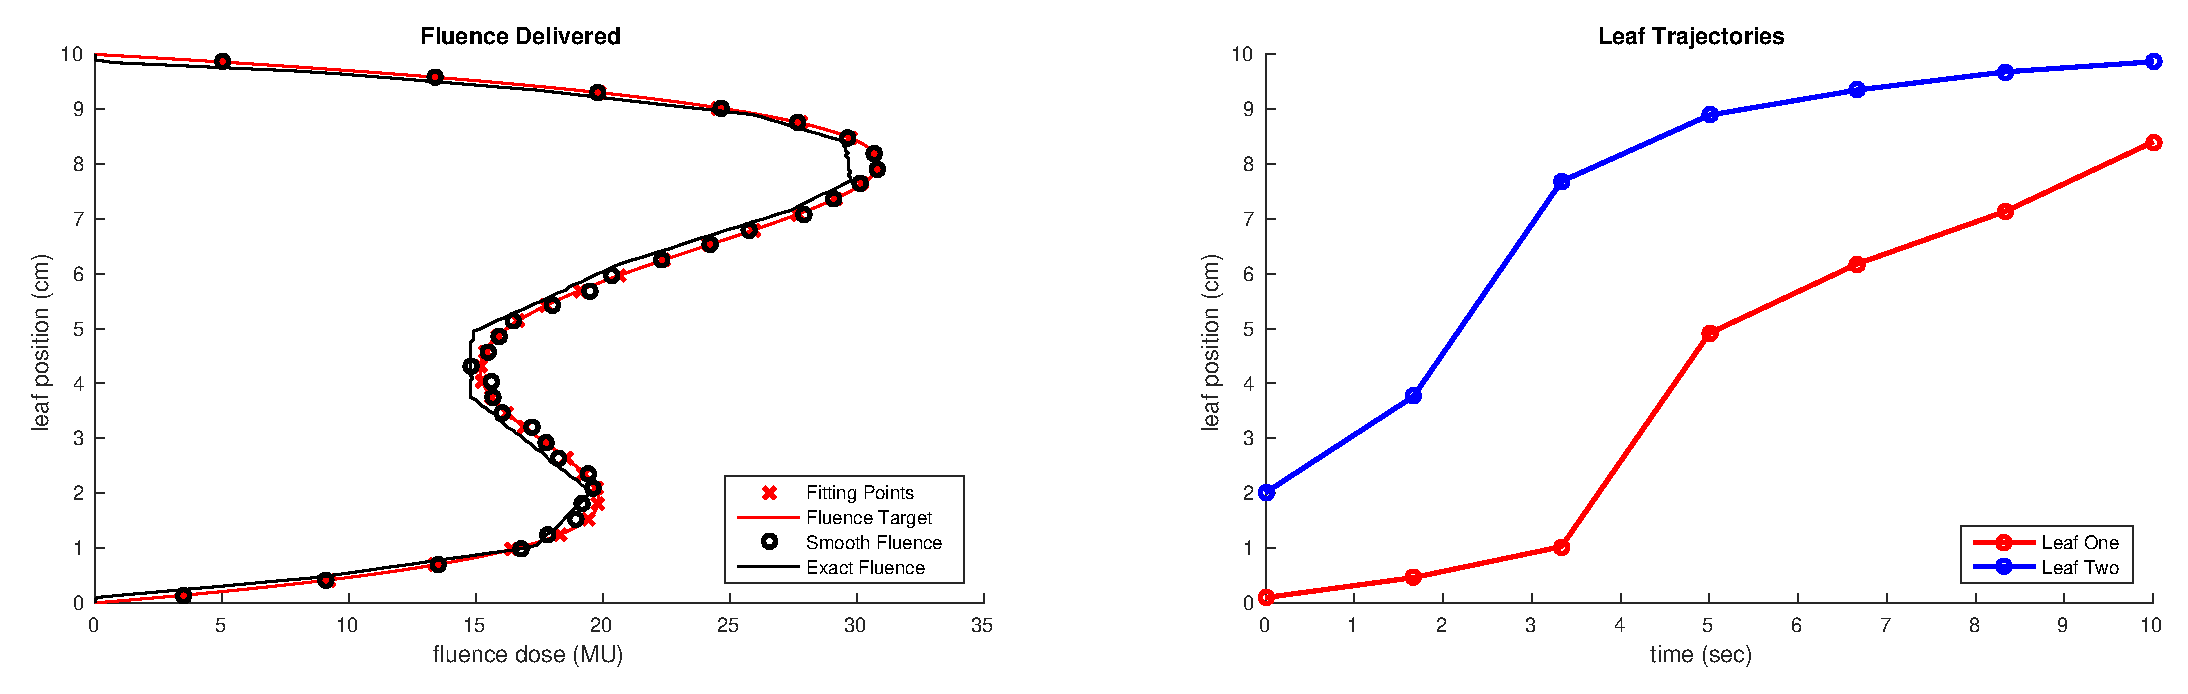
\includegraphics[width=\textwidth]{fig/fluenceMapSmoothingExample.pdf}
  \caption{ Optimal leaf-trajectories, computed with a smoothing width of 0.5 cm and a constant
            dose rate of 5.2 MU. Note the small discrepancy between the smooth model of the
            delivered fluence and the exact (no smoothing) model.}
  \label{fig:fluenceMapSmoothingExample}
\end{figure}


\subsection{Iterative Smoothing Refinement}

One common trick in trajectory optimization is to solve a trajectory optimization problem
iteratively, making small adjustments to the problem statement between each optimization,
and using the result of the previous optimization to seed the next.

We can do this iterative refinement with the leaf-blocking smoothing parameter,
starting with heavy smoothing and then using that solution to seed another optimization
with a smaller smoothing term.

We test this procedure by doing an experiment similar to the one discussed in
\S Section \ref{sec:LeafSmoothingComparison}, but using the solution of the heavy-smoothing
optimization to initialize the optimization with light smoothing.
Here we will use a sequence of three optimizations, starting with a smoothing of
0.5 cm, then moving to 0.1 cm, and finally 0.05 cm for the final optimization.

The resulting sweep of optimizations is shown in Figure \ref{fig:iterSmoothSweep}.
These results are better than either the heavy or light smoothing optimizations.
The total optimization time for all three optimizations is less than simply running the
light smoothing optimization from a niave guess, the model discrepancy is tiny, and the
solver is generally able to do a good job of avoiding local minima.

\begin{figure}
  \centering
  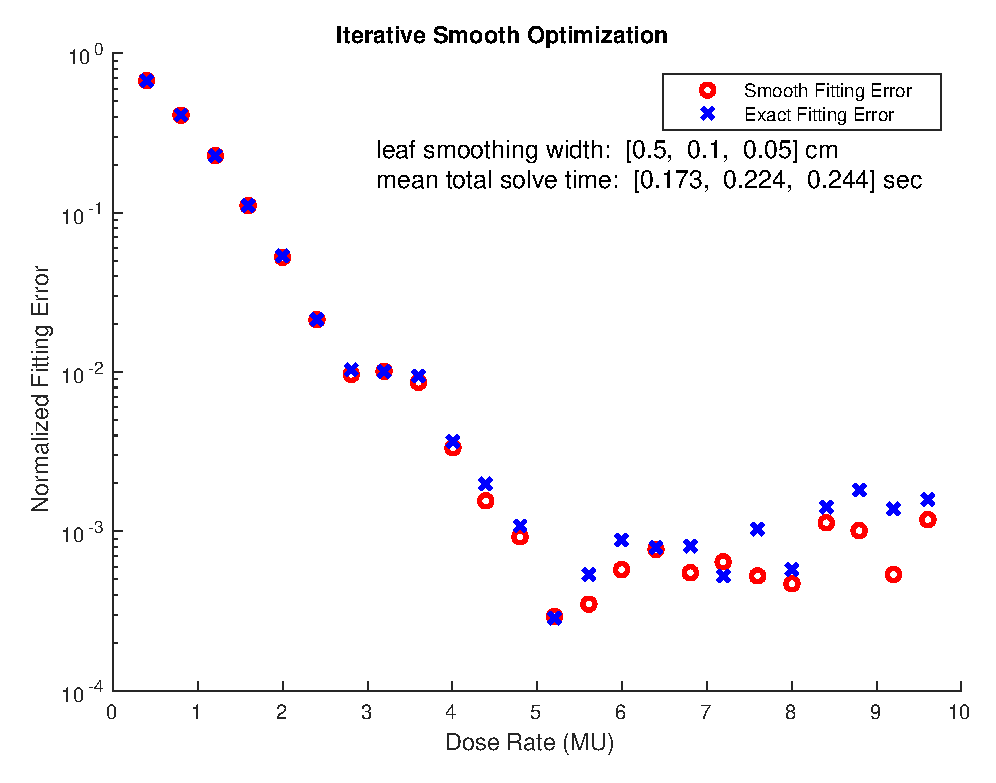
\includegraphics[width=3in]{fig/iterSmoothSweep.pdf}
  \caption{This plot shows the objective function value for the optimal leaf trajectories,
           given a constant fluence dose rate. Each optimization here is actually a set of three
           optimizations, each using a successively smaller smoothing distance. In all cases
           the first optimization used a smoothing distance of 0.5cm, the second used 0.1cm,
           and the final optimization used 0.05cm. This technique results in faster solve times
           than a single optimization with the smallest smoothing parameter, while also avoiding
           local minima.}
  \label{fig:iterSmoothSweep}
\end{figure}

Figure \ref{fig:fluenceMapIterativeBest} again shows the optimal leaf trajectories with a
constant dose rate of 5.2 MU. The leaf trajectories are qualitatively similar to those in
Figure \ref{fig:fluenceMapSmoothingExample}, but slight changes are present that make the
exact-model fluence profile much closer to the target profile.

\begin{figure}
  \centering
  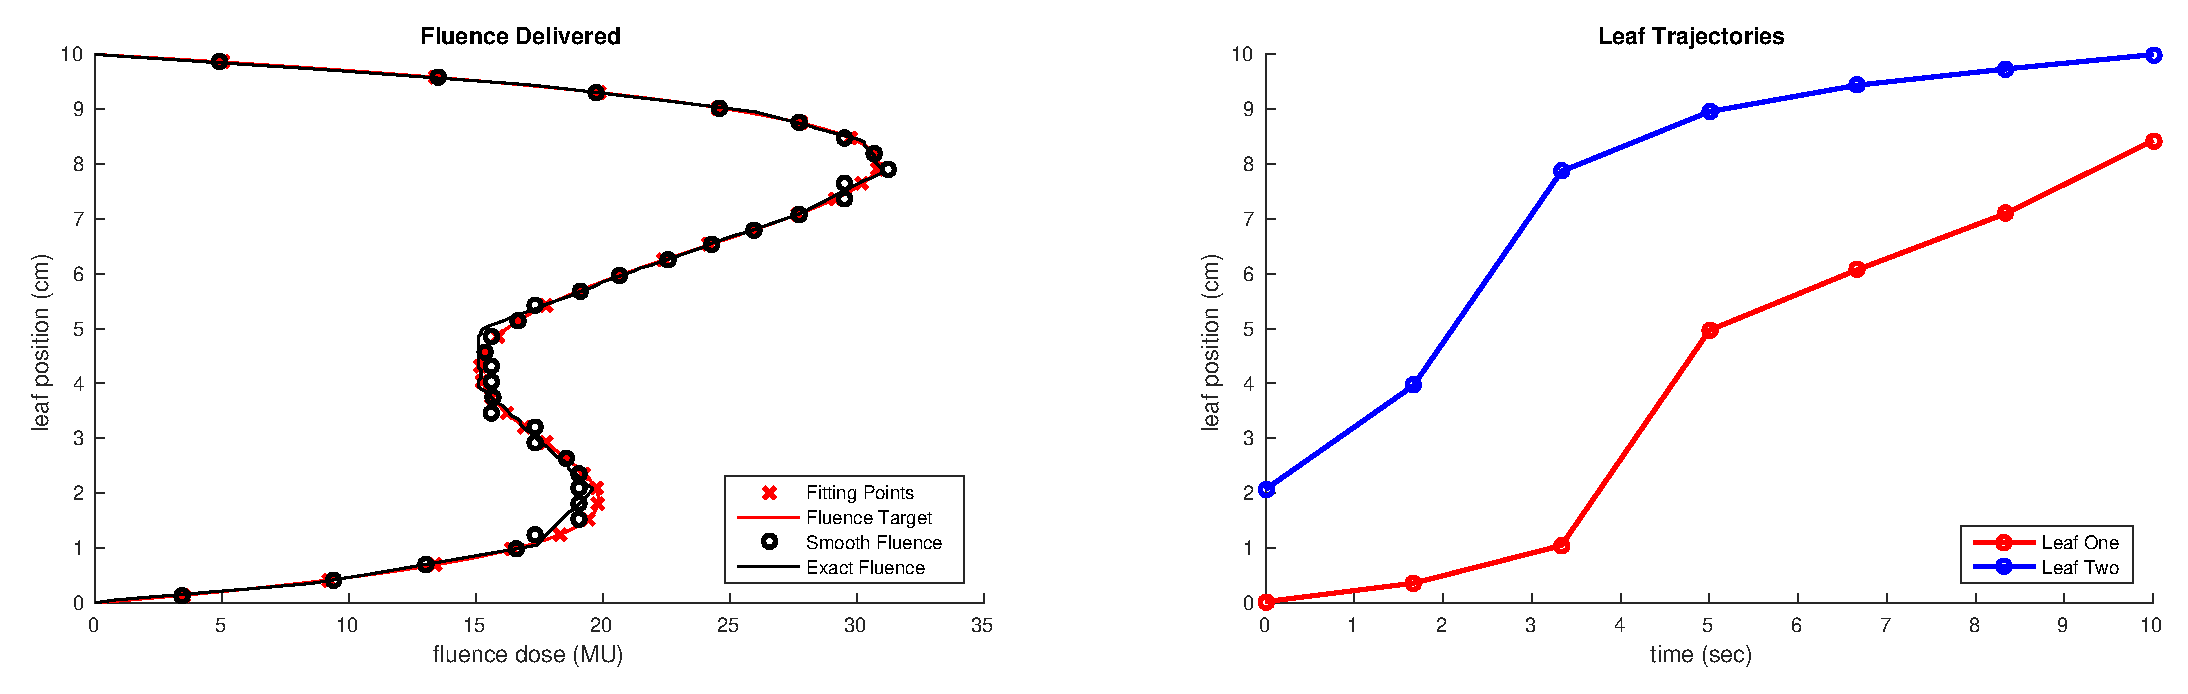
\includegraphics[width=\textwidth]{fig/fluenceMapIterativeBest.pdf}
  \caption{This plot shows the optimal leaf trajectories and delivered fluence map using the
           best solution (dose rate = 5.2 MU) found by the iterative optimization procedure.
           Note that these trajectories are similar to those in
           Figure \ref{fig:fluenceMapSmoothingExample}, but that the fitting is better here.}
  \label{fig:fluenceMapIterativeBest}
\end{figure}


\subsection{Computing Dose-rate Trajectories}

\todo{CMAES optimization for a single trajectory?}

\subsection{Multi-VMAT}

\todo{David - should we try to run an optimization with multiple pairs of leaves?}

\subsection{Misc. Notes:}

\todo{Clean up this section, perhaps add a few small plots.}

It seems that the velocity smoothing has little effect on the optimization: no significant
change observed in computation time, convergence, or trajectories.

The number of fitting points is important -- if there are too few the trajectories tend to
become less smooth and more local minima pop up. I believe that this is caused by overfitting.

The solve time varies linearly with number of trajectory segments, at least on the range of 7 to 13 segments.
The solution quality does not appear to change that much, although a few extra bumps do appear in the trajectories.
If there are too few points, then the it is sometimes not possible to capture some features in the target profile.

\section{Discussion and conclusions}


\subsection{Why first-order splines to represent trajectories?}
\label{sec:WhyUseLinearSplines}

In this section we informally discuss some of the design choices that were made when creating this
trajectory-based method for solving leaf and dose rate trajectories for fluence mapping.

\todo{This section should be edited to reduce length and needs some detailed citations.}

There are many ways to represent trajectories, and nearly all of them have associated transcription (optimization) methods.
In general there is one major trade-off:
use a larger number of low-order segments or
use a smaller number of high-order segments.

Selecting the correct method order typically comes down to problem specifics.
High-order methods are best when the system model is good and high accuracy is important.
The accuracy of these methods relies on the underlying problem being smooth over each
mesh interval, with few places where path constraints serve to shape the trajectory.
Low-order methods are best when the trajectory shape is dominated by path constraints and
high accuracy is not critical.
\todo{Cite my tutorial paper? Check if I discuss this in detail.
Also see if it is discussed in the reviews by Rao or Betts.}

Although our specific problem does not have path constraints, it does have a highly nonlinear objective function.
The smooth leaf-blocking model causes a strong nonlinearity in the objective function,
which would make careful mesh refinement necessary if high-order methods were used.
\todo{Cite GPOPS-II paper? Or perhaps Rao or Betts tutorial paper.}
We can avoid the need for careful mesh refinement by simply using a low-order model,
which also makes it easier to precisely handle the velocity and position limits on the leaf trajectories.

We did a few brief checks, comparing a few different schemes using cubic splines and compared them
to the linear spline presented in this paper. Although both methods worked, the linear spline methods
were much faster and were able to provide an good fit to the desired fluence profile.
One possible reason for the speed increase is that a set of three linear segments have less
coupling terms than a cubic spline fitting the same trajectory domain. The resulting sparsity in the
jacobian (derivative of the objective function) helps optimization. \cite{Betts}

The major drawback of a linear spline for leaf trajectories is that the resulting trajectory tends
to be less smooth, with a step change in velocity between each segment. This effect can be minimized
by using a large number of linear segments. In some cases this can lead to a slight numerical
instability, which is easily addressed by adding a small regularization term to the optimization,
minimizing the integral of the velocity-squared along the trajectory.


\subsection{Inner Optimization:  Leaf Trajectories}

\todo{Discuss figures in results section.}


\subsection{Outer Optimization:  Dose-Rate Trajectories}

\todo{Try doing a better job of performing two optimizations, and varying the leaf smoothing between them.
      See if this improves results.}

The outer optimization with CMAES works, but it still has the problem with local minima:
running the optimization N times produces several different solutions.
These solutions all have similar objective function values, but are created by different
dose rate trajectories.

It seems to me that the dose rate optimization has a large number of similar-valued minima,
since the leaf-trajectory optimization can find good solutions for most dose rate trajectories.
The residual fitting error seems to be more related to the choice of discretization -- number of
grid segments, rather than convergence failure.

I see two ways to go forward from here. First would be to try this optimization with a set of
leaf trajectories, to see if that helps force a better global solution, since the problem will
be more constrained. Second would be to play around more with global optimization and smoothing
terms.

If I make the smoothing term on the dose rate trajectory large, then I get repeatable solutions,
but they tend to be nearly-constant dose rate, and often relatively high.

Another option would be to modify the regularization term to include a  penalty on large
dose rates, which is perhaps desirable in the real system.



\bibliographystyle{unsrt}
\bibliography{all}

\end{document}
